\chapter{KHÁM PHÁ DỮ LIỆU, TIỀN XỬ LÝ VÀ BIỂU DIỄN ĐẶC TRƯNG}

\section{Phân tích khám phá dữ liệu (EDA)}

\subsection{Kích thước, kiểu dữ liệu và giá trị thiếu}

Sau khi đọc tệp với dấu phân tách tab và tắt cơ chế xử lý ngoặc kép (tin nhắn có thể chứa ký tự \texttt{"} không phải dấu bao trường), bộ dữ liệu có 5\,574 dòng và hai cột: \texttt{label} (chuỗi \textit{ham}/\textit{spam}) và \texttt{text} (chuỗi). Không có giá trị thiếu ở cả hai cột. Nhãn được mã hóa \texttt{ham}$\to0$, \texttt{spam}$\to1$ để spam là lớp dương.

\subsection{Tin nhắn trùng lặp}
\label{sec:eda-trung-lap}

Corpus gốc chứa \textbf{414 tin có nội dung trùng với một tin khác} (sau khi cắt khoảng trắng đầu/cuối), gồm 309 tin ham và 105 tin spam. Không có trường hợp cùng nội dung nhưng khác nhãn. Việc trùng lặp gây hai tác hại: làm sai lệch phân phối thật của dữ liệu, và nếu để cả hai bản sao ở hai phía của phép chia thì mô hình chỉ cần \textit{ghi nhớ} là đạt điểm cao trên test (rò rỉ). Nhóm \textbf{bỏ các bản trùng trước khi chia}, giữ lại một bản. Kết quả còn \textbf{5\,160 tin} (4\,518 ham, 642 spam).

\begin{table}[H]
\centering
\caption{Quy mô dữ liệu trước và sau khi loại bản trùng}
\label{tab:quy-mo}
\begin{tabular}{|p{5.4cm}|c|c|c|}
\hline
\textbf{Giai đoạn} & \textbf{Ham} & \textbf{Spam} & \textbf{Tổng} \\
\hline
Corpus gốc & 4\,827 & 747 & 5\,574 \\
\hline
Số tin trùng bị loại & 309 & 105 & 414 \\
\hline
Sau khi loại bản trùng & 4\,518 & 642 & 5\,160 \\
\hline
Tập huấn luyện (80\%) & 3\,614 & 514 & 4\,128 \\
\hline
Tập kiểm tra (20\%) & 904 & 128 & 1\,032 \\
\hline
\end{tabular}
\Nguon{Nhóm tính từ bộ dữ liệu SMS Spam Collection}
\end{table}

Phép chia $80/20$ có phân tầng theo nhãn nên tỉ lệ spam ở hai tập gần như bằng nhau (12,5\% ở tập huấn luyện và 12,4\% ở tập kiểm tra).

\subsection{Mất cân bằng lớp}
\label{sec:accuracy-lua-doi}

Spam chỉ chiếm \textbf{12,4\%} dữ liệu sau khi khử trùng lặp (Hình~\ref{fig:eda-balance}, bên trái). Hệ quả quan trọng: một ``mô hình'' luôn trả lời \textit{ham} sẽ đạt Accuracy $=904/1032\approx 87{,}6\%$ trên tập kiểm tra nhưng có Recall của lớp spam bằng 0; nó hoàn toàn vô dụng. Vì vậy Accuracy \textbf{không đủ} để đánh giá và báo cáo luôn kèm Precision, Recall và F1 của lớp spam.

\begin{figure}[H]
    \centering
    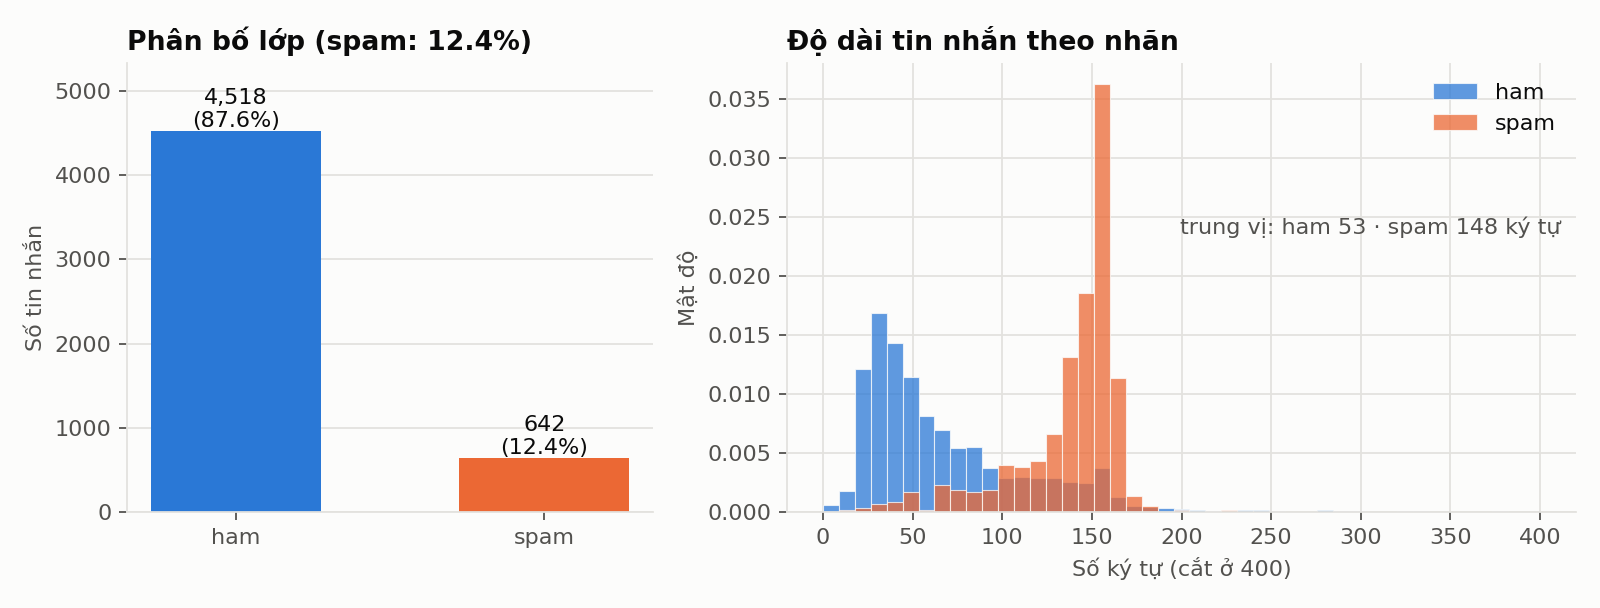
\includegraphics[width=\textwidth]{images/viz_1_class_balance.png}
    \caption{Phân bố lớp (trái) và phân bố độ dài tin nhắn theo nhãn (phải)}
    \label{fig:eda-balance}
    \Nguon{Nhóm xây dựng từ dữ liệu SMS Spam Collection (đã loại trùng)}
\end{figure}

\subsection{Độ dài tin nhắn}

Spam dài hơn rõ rệt: độ dài trung vị là \textbf{148 ký tự} (25 từ) so với \textbf{53 ký tự} (11 từ) của ham; trung bình lần lượt là 137,4 và 70,9 ký tự. Phân bố độ dài của spam tập trung thành một đỉnh nhọn quanh 150--160 ký tự, sát giới hạn 160 ký tự của một SMS, phản ánh việc spam thường được soạn sẵn để dùng trọn một tin nhắn (Hình~\ref{fig:eda-balance}, bên phải). Đây là đặc trưng mạnh, nhưng chồng lấn đáng kể ở vùng 100--150 ký tự nên không thể dùng riêng lẻ.

\subsection{Các đặc điểm cấu trúc gợi ý}

Nhóm khảo sát tỉ lệ tin chứa từng đặc điểm theo nhãn (Bảng~\ref{tab:dac-diem}).

\begin{table}[H]
\centering
\caption{Tỉ lệ tin nhắn chứa các đặc điểm cấu trúc theo nhãn}
\label{tab:dac-diem}
\begin{tabular}{|p{6.4cm}|c|c|}
\hline
\textbf{Đặc điểm} & \textbf{Spam (\%)} & \textbf{Ham (\%)} \\
\hline
Có ít nhất một chữ số & 93,9 & 15,8 \\
\hline
Có chuỗi từ 5 chữ số trở lên (số điện thoại, đầu số) & 76,5 & 0,1 \\
\hline
Có tên miền hoặc URL & 17,4 & 0,2 \\
\hline
Có ký hiệu tiền tệ (\textit{£}, \$, \texteuro) & 33,3 & 0,4 \\
\hline
Có từ viết hoa toàn bộ (từ 3 chữ cái trở lên) & 69,2 & 6,4 \\
\hline
Có dấu \texttt{!} & 47,0 & 11,7 \\
\hline
\end{tabular}
\Nguon{Nhóm tính trên 5\,160 tin sau khi loại trùng}
\end{table}

Bảng~\ref{tab:dac-diem} cho thấy chuỗi số dài, ký hiệu tiền và URL là tín hiệu gần như \textit{độc quyền} của spam. Đây là cơ sở thực nghiệm cho quyết định \textbf{không xóa số, tiền, URL} trong tiền xử lý mà thay bằng token đại diện (Mục~\ref{sec:tien-xu-ly}).

\subsection{Từ phổ biến theo lớp và giả thuyết ban đầu}

\begin{figure}[H]
    \centering
    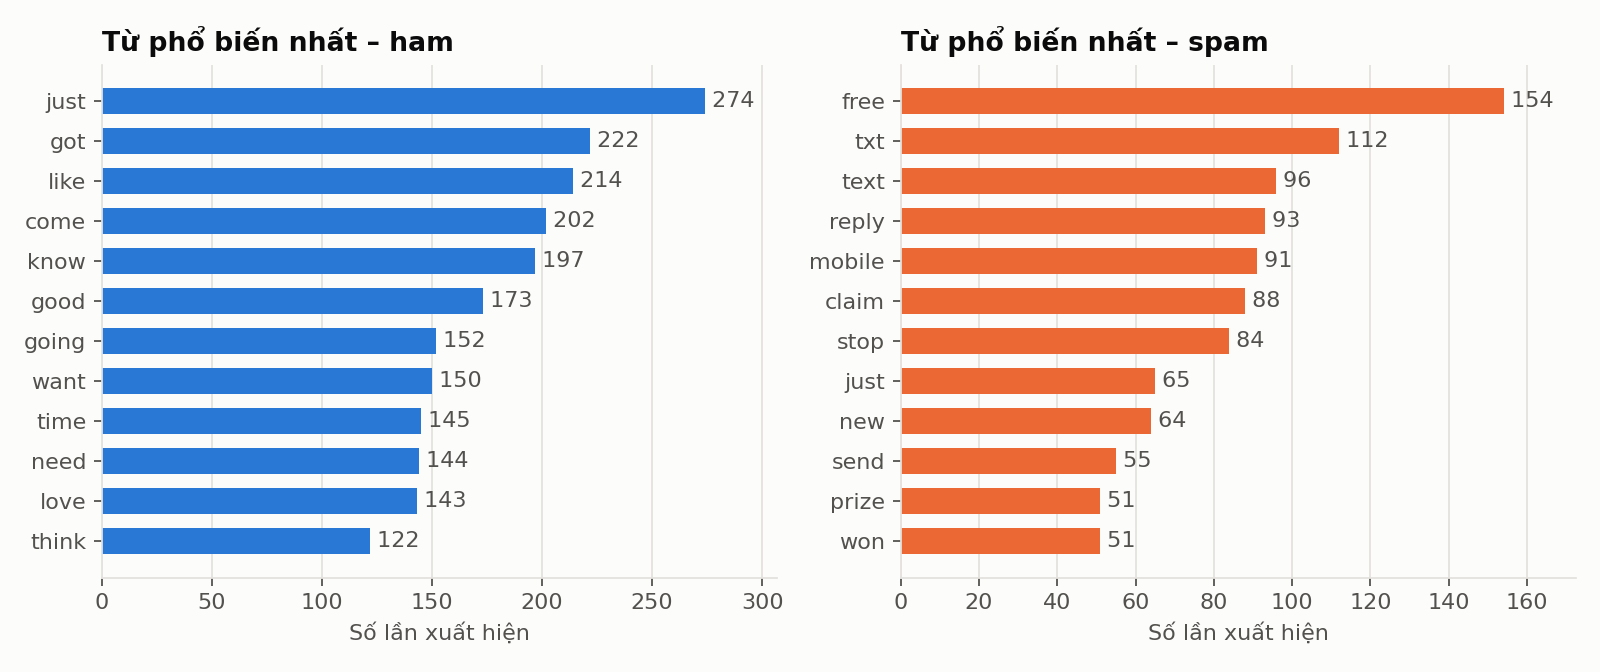
\includegraphics[width=\textwidth]{images/viz_2_top_words.png}
    \caption{Các từ phổ biến nhất của lớp ham (trái) và spam (phải), đã bỏ từ dừng}
    \label{fig:eda-topwords}
    \Nguon{Nhóm xây dựng từ dữ liệu SMS Spam Collection (đã loại trùng)}
\end{figure}

Từ phổ biến của ham là các từ hội thoại đời thường (\textit{just, got, like, come, know, love}), còn của spam là các từ kêu gọi hành động và khuyến mãi (\textit{free, txt, text, reply, mobile, claim, stop, prize, won}). Từ đó nhóm rút ra các \textbf{giả thuyết} để kiểm chứng ở các chương sau:

\begin{enumerate}[label=\textbf{H\arabic*.}]
    \item Từ khóa khuyến mãi và lời kêu gọi hành động là tín hiệu mạnh; một mô hình dựa trên đếm từ đã đạt chất lượng cao.
    \item Các cụm hai từ (\textit{to claim}, \textit{have won}) mang thêm thông tin so với từ đơn.
    \item Giữ lại tín hiệu số/tiền/URL (dưới dạng token) có lợi hơn xóa chúng; còn bỏ từ dừng có thể gây hại vì các từ như \textit{call}, \textit{to}, \textit{your} cũng mang tín hiệu.
\end{enumerate}

\section{Tiền xử lý văn bản}
\label{sec:tien-xu-ly}

\subsection{Nguyên tắc thiết kế}

Với bài toán spam, nhiều bước ``làm sạch'' kinh điển lại \textit{xóa mất tín hiệu}. Nhóm áp dụng ba nguyên tắc:

\begin{enumerate}[label=(\arabic*)]
    \item \textbf{Không xóa, mà thay thế bằng token.} URL, số tiền và số được thay bằng \texttt{urltoken}, \texttt{moneytoken}, \texttt{numtoken}. Các token này chỉ gồm chữ cái để không bị bước bỏ dấu câu/số xóa nhầm. Nhờ đó mô hình học được \textit{``có xuất hiện một URL/số tiền/số''} thay vì phải học từng giá trị cụ thể (mỗi số điện thoại hầu như chỉ xuất hiện một lần).
    \item \textbf{Mỗi bước phải bật/tắt độc lập} để làm thí nghiệm đối chứng (ablation) và có bằng chứng định lượng.
    \item \textbf{Bước tiền xử lý không học gì từ dữ liệu} (phương thức \texttt{fit} của \texttt{TextCleaner} không làm gì), vì vậy bản thân nó không thể gây rò rỉ.
\end{enumerate}

\subsection{Các bước và thứ tự áp dụng}

\begin{table}[H]
\centering
\caption{Các tùy chọn của bộ làm sạch văn bản \texttt{TextCleaner}}
\label{tab:cleaner}
\begin{tabular}{|c|p{3.6cm}|p{8.6cm}|}
\hline
\textbf{STT} & \textbf{Tùy chọn} & \textbf{Hành vi và lý do} \\
\hline
1 & \texttt{lowercase} (luôn bật) & Đưa về chữ thường để \textit{FREE} và \textit{free} là một. \\
\hline
2 & \texttt{replace\_url} & Thay URL/tên miền bằng \texttt{urltoken}; dấu câu cuối câu được giữ lại bên ngoài token. \\
\hline
3 & \texttt{replace\_money} & Thay mẫu tiền tệ (\textit{£900}, \textit{\$5}, \textit{50p}, \textit{10 pounds}) bằng \texttt{moneytoken}. Chạy trước bước số vì số tiền chứa chữ số. \\
\hline
4 & \texttt{replace\_number} & Thay mọi chuỗi chữ số còn lại bằng \texttt{numtoken}. \\
\hline
5 & \texttt{remove\_punct} & Thay ký tự không phải chữ/số/khoảng trắng bằng khoảng trắng. \\
\hline
6 & \texttt{remove\_stopwords} & Bỏ từ dừng tiếng Anh (danh sách của scikit-learn); mặc định tắt. \\
\hline
\end{tabular}
\Nguon{Nhóm xây dựng; mã nguồn \texttt{spam\_filter/preprocessing.py}}
\end{table}

Thứ tự (URL $\to$ tiền $\to$ số $\to$ dấu câu) có ý nghĩa: nếu bỏ dấu câu trước, \texttt{www.cashbin.co.uk} sẽ bị cắt thành năm mảnh vô nghĩa, còn nếu thay số trước thì \textit{£900} chỉ còn \textit{£numtoken}.

\subsection{Ví dụ minh họa}

Áp dụng lên tin nhắn mẫu \textit{``WINNER!! As a valued network customer you have been selected to receivea £900 prize reward! To claim call 09061701461. Claim code KL341. Valid 12 hours only.''}:

\begin{table}[H]
\centering
\caption{Đầu ra của bộ làm sạch với các cấu hình khác nhau}
\label{tab:vi-du-lam-sach}
\begin{tabular}{|p{3.4cm}|p{10.8cm}|}
\hline
\textbf{Cấu hình} & \textbf{Kết quả} \\
\hline
Chỉ chữ thường (E0--E4) & \textit{winner!! as a valued network customer you have been selected to receivea £900 prize reward! to claim call 09061701461. claim code kl341. valid 12 hours only.} \\
\hline
Token hóa URL/tiền/số và bỏ dấu câu (E5) & \textit{winner as a valued network customer you have been selected to receivea moneytoken prize reward to claim call numtoken claim code kl numtoken valid numtoken hours only} \\
\hline
Bỏ dấu câu và bỏ stopword (E6) & \textit{winner valued network customer selected receivea 900 prize reward claim 09061701461 claim code kl341 valid 12 hours} \\
\hline
\end{tabular}
\Nguon{Nhóm chạy trực tiếp lớp \texttt{TextCleaner}}
\end{table}

Có thể thấy cấu hình E5 biến số điện thoại 11 chữ số và mã \textit{KL341} (vốn là các token duy nhất, vô dụng khi mô hình gặp tin mới) thành các token chung \texttt{numtoken}, trong khi cấu hình E6 giữ nguyên chúng nhưng làm mất các từ như \textit{to}, \textit{you}, \textit{have}.

\section{Biểu diễn đặc trưng}

Hai phương án biểu diễn được cài đặt bằng \texttt{CountVectorizer} (BoW) và \texttt{TfidfVectorizer} (TF-IDF) của scikit-learn, với các tham số được thay đổi có kiểm soát (Bảng~\ref{tab:vectorizer}).

\begin{table}[H]
\centering
\caption{Các cấu hình vector hóa được khảo sát}
\label{tab:vectorizer}
\begin{tabular}{|p{3.6cm}|p{4.6cm}|p{5.8cm}|}
\hline
\textbf{Tham số} & \textbf{Giá trị khảo sát} & \textbf{Mục đích} \\
\hline
Loại biểu diễn & BoW, TF-IDF & Đếm thô so với có trọng số độ hiếm \\
\hline
\texttt{ngram\_range} & $(1,1)$, $(1,2)$ & Đo lợi ích của cụm hai từ \\
\hline
\texttt{min\_df} & 1, 2, 5 & Cân bằng giữa nhiễu và mất từ hiếm \\
\hline
\texttt{max\_df} & 0,9; 1,0 & Loại từ xuất hiện quá phổ biến \\
\hline
\end{tabular}
\Nguon{Nhóm xây dựng}
\end{table}

Từ vựng được xây dựng \textbf{chỉ từ tập huấn luyện}. Với cấu hình tốt nhất (TF-IDF bigram, \texttt{min\_df}=2, có token hóa), từ vựng gồm 9\,952 n-gram. Vector TF-IDF được chuẩn hóa $L_2$ theo mặc định.
